% [VERIFY] experiments -- experiments.md (E01-E06), evidence/tables/* + figures/* EXACT numbers.
% HONESTY: Fig.4/Fig.6 per-iteration curves NOT tabulated in Book -> trajectory claims hedged
%   ("the underlying analysis reports ... throughout training") and rendered figs are ENDPOINT bars/scatter
%   with caption disclaimers. No fabricated curves.
\section{Experiments}
\label{sec:exp}

\subsection{ImageNet Classification}
\label{sec:imagenet}
We evaluate our method on the ImageNet 2012 classification dataset that consists
of 1000 classes. The models are trained on the $1.28$ million training images
and evaluated on the $50{,}000$ validation images; we also obtain a final result
on the $100{,}000$ test images, reported by the test server. We evaluate both
top-1 and top-5 error rates.

\noindent\textbf{Plain networks vs.\ residual networks.}
We first evaluate 18-layer and 34-layer \plainnet{}s and their residual
counterparts under an identical training pipeline; the residual nets use
identity shortcuts with zero-padding for increasing dimensions (\optA), so they
have \emph{no extra parameter} compared to the \plainnet{} counterparts.
\Cref{tab:plain_vs_res} reports the top-1 validation error with 10-crop testing.
The 34-layer \plainnet{} has higher validation error ($28.54\%$) than the
18-layer \plainnet{} ($27.94\%$), exhibiting the \degrad{}: the deeper
\plainnet{} is worse despite its strictly larger solution space. The underlying
training-error analysis reports that the 34-layer \plainnet{}'s training error
remains higher than the 18-layer one's throughout the optimization, indicating
that this is an optimization difficulty rather than a final-step effect; per-iteration
curves are not reproduced here (see \cref{fig:plain_vs_res} and the limitation in
\cref{sec:conclusion}). The situation is reversed for the residual nets: the
34-layer ResNet attains $25.03\%$ top-1 error, which is $3.51$ points better than
the 34-layer \plainnet{} and $2.85$ points better than the 18-layer ResNet
($27.88\%$). This comparison verifies that residual learning removes the
\degrad{} and lets accuracy grow with depth at matched parameter count.

\begin{table}[t]
\centering
\caption{Top-1 error (\%, 10-crop testing) on ImageNet validation. Here the
ResNets have no extra parameter compared to their plain counterparts.
\emph{Source: Table 2 (\texttt{table2\_imagenet\_plain\_vs\_residual.md}); exact.}}
\label{tab:plain_vs_res}
\begin{tabular}{l c c}
\toprule
            & plain & ResNet \\
\midrule
18 layers   & 27.94 & 27.88 \\
34 layers   & 28.54 & \textbf{25.03} \\
\bottomrule
\end{tabular}
\end{table}

\begin{figure}[t]
\centering

\includegraphics[width=\linewidth]{figures/fig_imagenet_plain_vs_resnet.pdf}
\caption{ImageNet validation top-1 error (\%, 10-crop) for plain vs.\ residual
nets at 18 and 34 layers. \textbf{The 34-layer plain net degrades to $28.54\%$
while the 34-layer ResNet improves to $25.03\%$.} Bars are the reported
\emph{endpoint} validation errors from Table 2; the paper's per-iteration
training curves (Fig.~4) are not tabulated in the source artifact and are
therefore not redrawn here. N: single run per configuration (ImageNet val,
10-crop). \emph{Source: \texttt{table2\_imagenet\_plain\_vs\_residual.md}.}}
\label{fig:plain_vs_res}
\end{figure}

\noindent\textbf{Identity vs.\ projection shortcuts.}
We next examine projection shortcuts. \Cref{tab:shortcut} isolates the three
shortcut options on the 34-layer net against the \plainnet{} baseline:
(A) zero-padding identity shortcuts, parameter-free; (B) projection shortcuts
only for increasing dimensions, with all other shortcuts being identity; and
(C) projection shortcuts for all blocks. All three options are considerably
better than the \plainnet{} ($-3.51$ to $-4.35$ top-1 points). Among the three,
B is slightly better than A; we argue this is because the zero-padded
dimensions in A indeed have no residual learning. C is marginally better than B,
which we attribute to the extra parameters introduced by the thirteen
projection shortcuts. The small differences among A/B/C ($\le 0.65$ top-1 points)
indicate that projection shortcuts are not essential for addressing the
\degrad{}. We therefore do not use option C in the remainder of the paper, to
reduce memory/time complexity and model sizes; identity shortcuts are
particularly important for not increasing the complexity of the bottleneck
architectures introduced next.

\begin{table}[t]
\centering
\caption{ResNet-34 shortcut-option ablation on ImageNet validation (\%, 10-crop),
against the plain-34 baseline. \emph{Source: derived subset of Table 3
(\texttt{derived\_from\_table3\_shortcut\_options.md}); exact.}}
\label{tab:shortcut}
\small
\resizebox{\columnwidth}{!}{%
\begin{tabular}{l l c c c}
\toprule
model & shortcut & top-1 & top-5 & $\Delta$ top-1 \\
\midrule
plain-34    & none                 & 28.54 & 10.02 & --- \\
ResNet-34 A & identity + zero-pad   & 25.03 & 7.76 & $-3.51$ \\
ResNet-34 B & proj.\ on dim.\ change & 24.52 & 7.46 & $-4.02$ \\
ResNet-34 C & proj.\ everywhere      & 24.19 & 7.40 & $-4.35$ \\
\bottomrule
\end{tabular}}
\end{table}

\noindent\textbf{Going deeper with bottleneck blocks.}
Using the bottleneck design (\cref{sec:bottleneck}), we construct 50-, 101-, and
152-layer residual nets with option B shortcuts and train them with the same
recipe. \Cref{tab:val_full} reports the full 10-crop validation errors against
contemporary \plainnet{} and competitor baselines. The top-1 error decreases
monotonically with depth, from $24.52\%$ (ResNet-34 B) to $22.85\%$, $21.75\%$,
and $21.43\%$ for ResNet-50, ResNet-101, and ResNet-152 respectively, with the
matching top-5 error falling from $7.46\%$ to $5.71\%$. Because residual blocks
add no parameters relative to their plain counterparts, this gain within the
studied depths is attributable to depth rather than added width.
\Cref{fig:depth} plots the trend. The deeper bottleneck nets also remain
efficient: ResNet-152 has $11.3\times10^{9}$ FLOPs (\cref{tab:arch}), still below
VGG-16/19.

\begin{table}[t]
\centering
\caption{Error rates (\%, 10-crop testing) on ImageNet validation. VGG-16 is
based on our test. ResNet-50/101/152 are of option B that only uses projections
for increasing dimensions. \emph{Source: Table 3
(\texttt{table3\_imagenet\_validation\_full.md}); exact.}}
\label{tab:val_full}
\small
\begin{tabular}{l c c}
\toprule
model & top-1 err. & top-5 err. \\
\midrule
VGG-16~\cite{vgg2015}        & 28.07 & 9.33 \\
GoogLeNet~\cite{googlenet2015} & ---   & 9.15 \\
PReLU-net~\cite{msra2015}    & 24.27 & 7.38 \\
plain-34                     & 28.54 & 10.02 \\
ResNet-34 A                  & 25.03 & 7.76 \\
ResNet-34 B                  & 24.52 & 7.46 \\
ResNet-34 C                  & 24.19 & 7.40 \\
ResNet-50                    & 22.85 & 6.71 \\
ResNet-101                   & 21.75 & 6.05 \\
ResNet-152                   & \textbf{21.43} & \textbf{5.71} \\
\bottomrule
\end{tabular}
\end{table}

\begin{figure}[t]
\centering
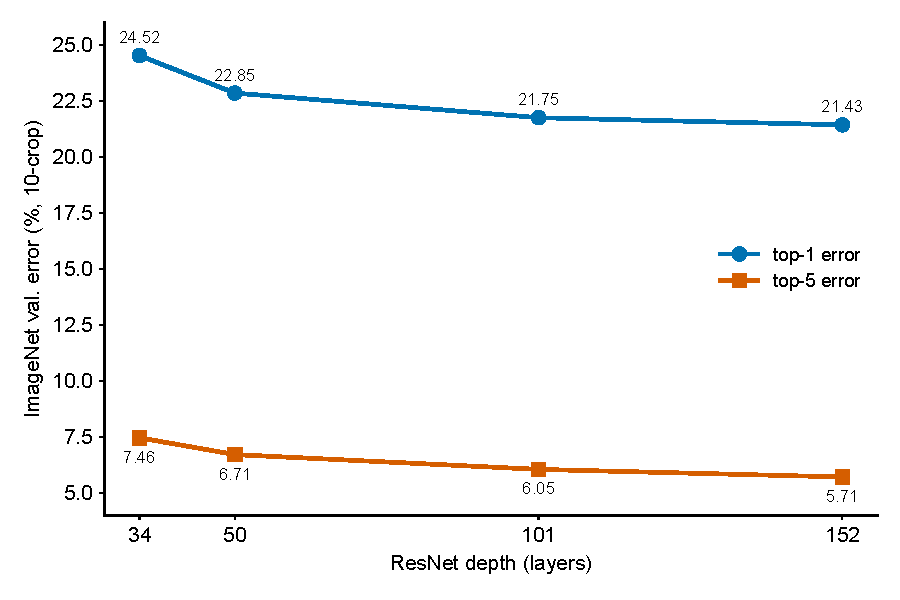
\includegraphics[width=\linewidth]{figures/fig_imagenet_depth_scaling.pdf}
\caption{ImageNet validation error (\%, 10-crop) of residual nets vs.\ depth.
\textbf{Top-1 error falls monotonically from $24.52\%$ at 34 layers to
$21.43\%$ at 152 layers.} Markers are reported endpoint errors from Table 3
(ResNet-34 shown as option B). N: single run per depth (ImageNet val, 10-crop).
\emph{Source: \texttt{table3\_imagenet\_validation\_full.md}.}}
\label{fig:depth}
\end{figure}

\noindent\textbf{Single-model and ensemble results.}
With multi-scale fully-convolutional testing, the single-model ResNet-152
reaches $19.38\%$ top-1 / $4.49\%$ top-5 error on the validation set, the best
single-model result among the entries in \cref{tab:singlemodel} and below the
prior PReLU-net and BN-inception single models. Finally, an ensemble of six
models of different depth attains $\mathbf{3.57\%}$ top-5 error on the ImageNet
\emph{test} set (\cref{tab:ensemble}), which won the 1st place in the ILSVRC 2015
classification competition.

\begin{table}[t]
\centering
\caption{Single-model results on the ImageNet validation set
(except $\dagger$ reported on the test set). \emph{Source: Table 4
(\texttt{table4\_imagenet\_singlemodel.md}); exact, caption qualifier preserved.}}
\label{tab:singlemodel}
\small
\begin{tabular}{l c c}
\toprule
method & top-1 err. & top-5 err. \\
\midrule
VGG~\cite{vgg2015} (ILSVRC'14)       & ---   & $8.43\dagger$ \\
GoogLeNet~\cite{googlenet2015} (ILSVRC'14) & --- & 7.89 \\
VGG~\cite{vgg2015} (v5)              & 24.4  & 7.1  \\
PReLU-net~\cite{msra2015}           & 21.59 & 5.71 \\
BN-inception~\cite{bn2015}          & 21.99 & 5.81 \\
ResNet-34 B                          & 21.84 & 5.71 \\
ResNet-34 C                          & 21.53 & 5.60 \\
ResNet-50                            & 20.74 & 5.25 \\
ResNet-101                           & 19.87 & 4.60 \\
ResNet-152                           & \textbf{19.38} & \textbf{4.49} \\
\bottomrule
\end{tabular}
\end{table}

\begin{table}[t]
\centering
\caption{Error rates (\%) of ensembles. The top-5 error is on the test set of
ImageNet and reported by the test server. \emph{Source: Table 5
(\texttt{table5\_imagenet\_ensembles.md}); exact.}}
\label{tab:ensemble}
\small
\begin{tabular}{l c}
\toprule
method & top-5 err.\ (test) \\
\midrule
VGG~\cite{vgg2015} (ILSVRC'14)      & 7.32 \\
GoogLeNet~\cite{googlenet2015} (ILSVRC'14) & 6.66 \\
VGG~\cite{vgg2015} (v5)             & 6.8  \\
PReLU-net~\cite{msra2015}          & 4.94 \\
BN-inception~\cite{bn2015}         & 4.82 \\
\textbf{ResNet (ILSVRC'15)}         & \textbf{3.57} \\
\bottomrule
\end{tabular}
\end{table}

\subsection{CIFAR-10 and Analysis}
\label{sec:cifar}
We conducted more studies on the CIFAR-10 dataset, which consists of $50{,}000$
training and $10{,}000$ testing images in 10 classes. The CIFAR networks use a
$6n{+}2$ stacked-layer skeleton with $\{16,32,64\}$ filters across the three
$\{32,16,8\}$ feature-map sizes, and option A identity shortcuts everywhere, so
the residual nets have exactly the same depth, width, and number of parameters
as the plain counterparts. \Cref{tab:cifar} reports the test error against
baselines. The residual nets improve as depth grows from 20 to 110 layers, with
test error decreasing $8.75 \to 7.51 \to 7.17 \to 6.97 \to 6.43\%$; the 110-layer
ResNet ($1.7$M parameters) reaches $6.43\%$ (best; mean$\pm$std $6.61\pm0.16$
over 5 runs), competitive with far larger prior models. \Cref{fig:cifar} plots
the trend, including the 1202-layer point discussed below. The corresponding
\plainnet{}s, by contrast, suffer from the \degrad{} as depth increases, and the
110-layer \plainnet{} reaches an error higher than $60\%$ and is not displayed.

\noindent\textbf{Warmup for the 110-layer net.}
For the 110-layer ResNet, an initial learning rate of $0.1$ is slightly too
large to start converging. We therefore warm up the training with a learning
rate of $0.01$ for the first $\sim 400$ iterations until the training error drops
below $\sim 80\%$, and then restore the learning rate to $0.1$ to continue. The
remaining schedule is unchanged. We note this warmup is a stability heuristic
specific to this depth rather than a fundamental requirement of residual
learning.

\noindent\textbf{Exploring over 1000 layers.}
We further explore an aggressively deep model of 1202 layers ($19.4$M
parameters). Our method shows no optimization difficulty at this depth, and the
1202-layer net achieves a training error below $0.1\%$. Its test error, however,
is $7.93\%$ --- worse than the 110-layer net (\cref{tab:cifar},
\cref{fig:cifar}). We argue this is because of overfitting: the 1202-layer
network is unnecessarily large for this small dataset, and we did not use strong
regularization such as maxout or dropout in this work. The result is reported
as a study of optimization behavior at extreme depth, not as a recommended
operating point.

\begin{table}[t]
\centering
\caption{Classification error on the CIFAR-10 test set. All methods are with
data augmentation. For ResNet-110, we run it 5 times and show ``best (mean
$\pm$ std)''. \emph{Source: Table 6 (\texttt{table6\_cifar10.md}); exact,
caption qualifier preserved.}}
\label{tab:cifar}
\small
\resizebox{\columnwidth}{!}{%
\begin{tabular}{l r r l}
\toprule
method & \#layers & \#params & error (\%) \\
\midrule
Maxout~\cite{maxout2013}      & ---  & ---    & 9.38 \\
NIN~\cite{nin2013}            & ---  & ---    & 8.81 \\
DSN~\cite{dsn2014}            & ---  & ---    & 8.22 \\
\midrule
FitNet~\cite{fitnets2015}     & 19   & 2.5M   & 8.39 \\
Highway~\cite{highway2015,highwaydeep2015} & 19 & 2.3M & 7.54 (7.72 $\pm$ 0.16) \\
Highway~\cite{highway2015,highwaydeep2015} & 32 & 1.25M & 8.80 \\
ResNet                        & 20   & 0.27M  & 8.75 \\
ResNet                        & 32   & 0.46M  & 7.51 \\
ResNet                        & 44   & 0.66M  & 7.17 \\
ResNet                        & 56   & 0.85M  & 6.97 \\
ResNet                        & 110  & 1.7M   & \textbf{6.43 (6.61 $\pm$ 0.16)} \\
ResNet                        & 1202 & 19.4M  & 7.93 \\
\bottomrule
\end{tabular}}
\end{table}

\begin{figure}[t]
\centering
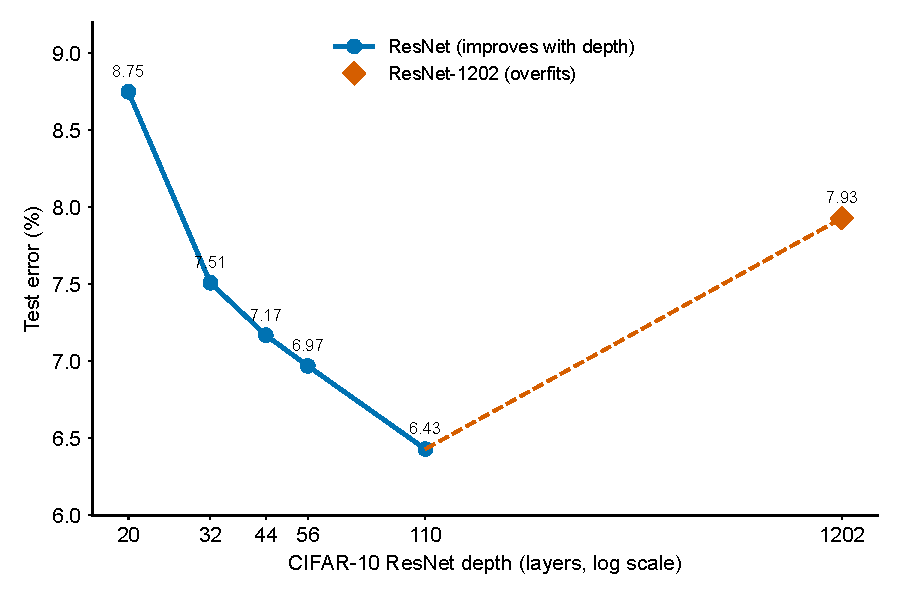
\includegraphics[width=\linewidth]{figures/fig_cifar_depth.pdf}
\caption{CIFAR-10 test error vs.\ ResNet depth. \textbf{Test error improves from
$8.75\%$ at 20 layers to $6.43\%$ at 110 layers, then rises to $7.93\%$ at 1202
layers due to overfitting.} Markers are reported endpoint test errors from
Table 6 (the 110-layer point is the 5-run best). N: 5 runs for ResNet-110, single
run otherwise. \emph{Source: \texttt{table6\_cifar10.md}.}}
\label{fig:cifar}
\end{figure}

\subsection{Object Detection on PASCAL and COCO}
\label{sec:detection}
Our method has good generalization performance on other recognition tasks. We
adopt the baseline Faster R-CNN detection framework and study only the effect of
replacing the VGG-16 backbone with ResNet-101, holding the detection
hyperparameters fixed. \Cref{tab:voc} reports PASCAL VOC results: mAP improves
from $73.2$ to $76.4$ on VOC 2007 (trained on 07+12) and from $70.4$ to $73.8$ on
VOC 2012 (trained on 07++12). On COCO (\cref{tab:coco}), the standard
mAP@$.5$ improves from $41.5$ to $48.4$, and the stricter mAP@$[.5,.95]$ --- which
rewards tighter localization --- improves from $21.2$ to $27.2$. This $6.0$-point
absolute gain is a $28\%$ relative improvement, and is comparable to the gain on
the looser mAP@$.5$, indicating that the deeper representations help both
recognition and localization. Because only the backbone changed, the improvement
is attributable to the learned representation rather than the detection pipeline.

\begin{table}[t]
\centering
\caption{Object detection mAP (\%) on the PASCAL VOC 2007/2012 test sets using
baseline Faster R-CNN. \emph{Source: Table 7
(\texttt{table7\_pascal\_voc\_detection.md}); exact.}}
\label{tab:voc}
\small
\resizebox{\columnwidth}{!}{%
\begin{tabular}{l c c}
\toprule
 & 07+12 (VOC 07 test) & 07++12 (VOC 12 test) \\
\midrule
VGG-16     & 73.2 & 70.4 \\
ResNet-101 & \textbf{76.4} & \textbf{73.8} \\
\bottomrule
\end{tabular}}
\end{table}

\begin{table}[t]
\centering
\caption{Object detection mAP (\%) on the COCO validation set using baseline
Faster R-CNN. \emph{Source: Table 8 (\texttt{table8\_coco\_detection.md}); exact.}}
\label{tab:coco}
\small
\begin{tabular}{l c c}
\toprule
 & mAP@$.5$ & mAP@$[.5,.95]$ \\
\midrule
VGG-16     & 41.5 & 21.2 \\
ResNet-101 & \textbf{48.4} & \textbf{27.2} \\
\bottomrule
\end{tabular}
\end{table}
